%!TEX root = thesis.tex

%
%==========================================================================================
%
\chapter{Activity Recognition}
\label{chap:activity_recognition}
\index{activity recognition}
Activity recognition is an underpinning task in behavior analysis. It transforms sensor data to a higher-level description of behavior primitives. This chapter presents a pipeline for recognizing an agent's atomic activities from multidimensional, sequential, spatio-temporal data. We first formulate the problem and discuss the basic ideas, followed by a description of the pipeline components, including noise filtering (Section~\ref{sec:ar:noise}), designing feature vectors and model learning (Section \ref{sec:ar:ml}), and providing recognized activity continuity (Section~\ref{sec:ar:spurious}). In addition, we present approaches for recognizing compound activities and activities that result from interactions among agents (Section~\ref{sec:ar:interactions}). %Finally, a brief discussion of the proposed algorithms concludes the chapter.

%We first formulate the problem and discuss our basic ideas in Section~\ref{sec:ar:problem}, followed by description of our proposed filtering algorithm for location-based sensors. Next, we descrei


\section{Problem Statement and Basic Ideas}
\label{sec:ar:problem}

Observing an agent's atomic activities is relatively straightforward in domains with discrete states. For example, observing a person on a computer terminal consists of typing a command that changes the state; hence, an atomic action corresponds to a command. Other continuous domains, where an agent is observed with sensors providing sequential numerical data, require more steps, since these sequences are not automatically labeled with activities. The main problem is how to segment sequences into atomic activities.

Consider an environment where the movement of an agent is observed with several sensors providing measurements at each time step $t$.
\index{observation}
\begin{definition}
\label{def:observation}
	\emph{Observation vector} $\mathbf{x}_t$ is a multi-dimensional signal vector containing stochastic values from each sensor at a given time point $t$. 
\end{definition}
\noindent At this point, we assume that it is possible to construct an observation from all the sensors regardless of the frequency with which a particular sensor provides measurements.

\index{observation!observation sequence}
\begin{definition}
\label{def:observation_vector}
	\emph{Observation sequence} $\mathbf{X}$ consists of $T$ observation measurements such that $\mathbf{X}=\{ \mathbf{x}_t | 1 \leq t \leq T \}$.
\end{definition}

%\begin{definition}
%\label{def:observation_vector}
%	\emph{Action sequence} $X$ consist from $T'$ actions observation measurements s.t. $X=\{x_t | 1 \leg t \leq t\}$.

Given a finite set of possible activities $\mathbb{A}=\{a_1, ..., a_K\}$, our  goal is to automatically segment an observation sequence $\mathbf{X}=\{\mathbf{x}_1, ..., \mathbf{x}_T\}$ into a sequence of activities $\{a_1, ..., a_{T}\}$. %, more precisely, to assign an activity to each observation $\mathbf{x}_t$. 
In the literature, activity is often referred to as action, activity, complex activity, compound task, goal, or plan. The main difference is how many observations are used to assign an activity. We define activity as behavior in a specific time span, as follows:
\begin{definition}
\label{def:activity}
\index{activity}
	\emph{Activity} $a_{i, j} \in \mathbb{A}$ describes an action as behavior caused by an agent in a particular situation limited by time span $i \leq t \leq j$ that explains observations $\mathbf{x}_i, ..., \mathbf{x}_j$, where $\mathbb{A}$ is a set of possible activities.
\end{definition}

A special case is when activity corresponds to a single observation; that is, $a_{i,i}$. We denote such activity as atomic action.
\begin{definition}
\label{def:action}
\index{action!atomic action}
	\emph{Atomic action} $a_t \in \mathbb{A}$ at time step $t$ is an activity from a set of possible activities $\mathbb{A}$ assigned to an observation $\mathbf{x}_t$ with function  
	$$
	f: \mathbb{R}^{|\mathbf{x}|} \rightarrow \mathbb{A}.
	$$
\end{definition}

However, in general, the number of observations described by an activity is not fixed, since different behaviors require a different number of observations, and behavior itself can be presented at different granularities. For example, behavior {\it breakfast routine} can be an activity itself, or it can be segmented into several activities, for example, {\it making coffee}, {\it putting food on the table}, {\it eating}, and {\it cleaning}.

Labeling multi-dimensional time-series sensor data is inherently more complex than classifying traditional, nominal data that contain little noise. First, each observation is temporally connected to the previous and next observations, making it very difficult to apply a straightforward classification of a single observation only. Second, the data obtained by sensors at different time points are stochastic due to sensor noise, environmental disturbances, and many other reasons. Moreover, an activity can comprise various sub-activities executed in different manners, resulting in high intra-class differences. Finally, all these reasons make an activity recognition model imprecise, resulting in unseen observation vectors being mislabeled. Therefore, it is highly desirable to ensure continuity and consistency in the recognized activity sequence.

\index{activity recognition pipeline}
To deal with the above-mentioned challenges, we propose an activity-recognition pipeline, referred to as ARPipe, as shown in Figure~\ref{fig:ar:pipeline}. We first devise a noise removal phase, which is strongly tightened with the type of sensors deployed in the domain; then we show an approach based on location-based sensors attached to the human body. The next phase extracts domain-dependent features from a set of observations and constructs a feature vector, which is used in the next step. Based on the feature vector, an activity recognition model assigns an atomic action to each observation. Finally, transitions between activities that cannot occur in reality are removed in the last step.
\index{activity recognition!activity recognition pipeline}

\begin{figure}[!ht]
\centering
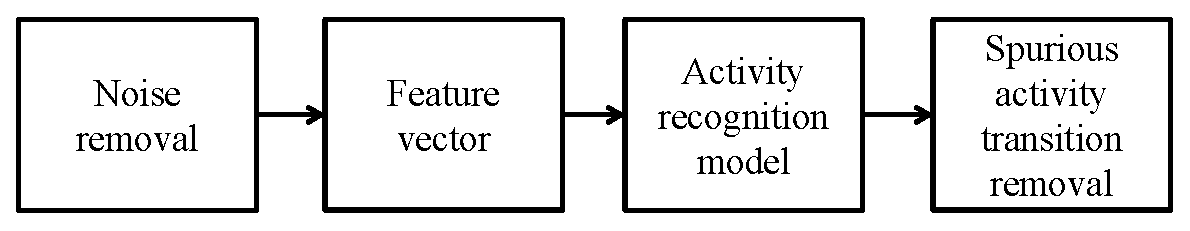
\includegraphics[width=0.9\linewidth]{chap_AR/ARPIPE}
\caption{ARPipe, an activity recognition pipeline.}
\label{fig:ar:pipeline}
\end{figure}

The activity recognition model is constructed with a supervised learning approach, which consists of training and classification steps. In the training step, a set of labeled data is provided to train the model. The second step is used to assign a label to new, unseen data by the trained model. The data in both phases must be pre-processed with the same set of tools, such as filtering and feature vector computation. 

The post-processing phase; that is, spurious activity removal, can also be a model itself and, hence, also requires a learning step. In this case, the pre-processing step also includes activity recognition. Therefore, it is important that the dataset used for training is not the same as that used for the training activity recognition model.


The first two phases in the proposed pipeline are domain-dependent, while the last two phases are general. We demonstrate our methods in the ambient-assisted living domain (see Chapter~\ref{chap:confidence}) to recognize activities performed by an elderly person in a home environment, wearing location-based tags that provide absolute three-dimensional coordinates. The goal is to label an observation vector with eight atomic actions. Specifically, we present two approaches for filtering and feature vector construction to illustrate how they can be used to robustly recognize activities in the presence of noise, clutter, and human action execution variability.



%\section{Motivating Domain}
%\label{sec:ar:problem}


\section{Dealing with Noise}
\label{sec:ar:noise}

\index{noise removal}
An important sensor technology that makes human activity recognition possible relies on real-time location systems (RTLSs). They provide three-dimensional coordinates of tags attached to the human body. High-fidelity optical system, such as \cite{Vicon2009} and SMART \citep{SMART2009}, provide accurate measurements ($\pm 2$ mm), but often include outliers due to marker occlusion and mislabeling. Furthermore, they require a line-of-sight between the body-attached tags and the cameras. They are good for lab use, but fail in real-world applications as they are usually too expensive, hard to install, and have limitations, such as line-of-sight or a confined operational area. More affordable systems rely on radio technology, which is less obtrusive and cheaper, but less accurate. Systems based on ultra-wideband technology (UWB), such as Ubisense~\citep{Ubisense}, achieve $\pm 15$ cm accuracy in an ideal setting, which makes human activity recognition challenging. The main problem addressed in this section is how to de-noise human-motion trajectories captured with UWB RTLS in order to improve activity recognition.

We demonstrate noise filtering on Ubisense, a commercially available localization system. Ubisense allows local positioning by tracking a set of reasonably small tags, which are attached to a person's body. A sampling frequency of around 10 Hz can be achieved with up to four tags attached to a person simultaneously. Each tag maintains radio contact with a stationary sensor (for example, mounted on the wall). These sensors and tags communicate using UWB radio technology. Both the time arrival difference and the radio signal arrival angle are used to calculate the tag position. In a typical open environment, a location accuracy $\pm$15 cm can be achieved across 95\% of the readings. However, in real-life scenarios the accuracy occasionally exceeds $\pm$ 200 cm, which represents quite a challenge for preprocessing and filtering. 

%Generally, more tags worn by a person enables more accurate activity recognition; however, given large enough noise, even an increased number of tags does not necessarily improve the results. For example, it turns out that the accuracy of the activity-recognition model was comparable when using only eight or four tags [ref]. However, having less than two tags significantly impacts the activity recognition accuracy. Since more tags require more effort from the person, it is desirable to use as little tags as possible. It this section we show an approach using four tags attached to at the following locations on the body (as shown in Figure~\ref{fig:tags}): chest, waist (optional), left and right ankles.

De-noising human motion captured with UWB sensors raises several challenges. First, motion-capture data may contain a certain percentage of missing values due to packet loss, temporal sensor disability, low battery, etc. Second, due to sensor noise and environment disturbances, motion-capture data often include outliers and unstable measurements, which corrupt body posture reconstruction. This results in a violation of physical body constraints as well as spatio-temporal body constraints, which in turn introduces additional noise into the activity recognition models. Finally, essential activity recognition features that are computed from noisy measurements (for example, velocity, acceleration) may have an integral error term; that is, the error accumulates over time.

In this section, we propose an efficient approach for de-noising human-motion trajectories that not only filters corrupted motion data, but also enforces the human body's spatio-temporal constraints and enables more accurate feature computation. The key idea is to construct a series of filters that addresses the above-mentioned challenges.

% :\\
% (i) median\\
% (ii) body\\
% (iii) Kalman\\
% (iv) adaptive low-pass  

%
%	? vrstni red filtrov
%	? body filter kot kalmanov filter
%	mediana (B)
%	body filter (B)
%	kalmanov filter (izracuna tudi hitrosti, ki jih ne merimo direktno = feature za ML) (B prpi?i)
%	is moving (R predelaj)
%	low pass filter (R+B)
%	setting parametters:
%		mediana: dolzina okna
%		body: izmeri cloveka
%		kalman: std odkloni iz analize suma
%		is moving: iz analize suma
%		low-pass: parameter za nastavljanje lambde


% In this section we introduce a set of filters that address...

\subsection{Dealing with Outliers}
\label{sec:ar:noise:median}

% Idea: weighted median filter \cite{Yin1996median}

Median filter is a non-linear filter that can suppress impulsive, isolated noise without blurring sharp changes in the signal \citep{Yin1996median}. The filter consists of a sequential sample window with odd length $w=2n+1$. At each time step $t$, the filter returns the median of the elements in the window:
\begin{equation}
	x_t' = \text{median}(x_{t-n}, ..., x_t, ..., x_{t+n}).
\end{equation}

The only parameter of the median filter is the window length $w$, which introduces a delay of length $\lfloor w/2 \rfloor$. A larger window size may smooth the signal too much, while a smaller window size may not remove the high density noise. A common approach is to choose a window length such that desired signal features are preserved while attenuating noise.

%The majority of computational time is spent on calculating the media of each window, hence an efficient median calculation is crucial for the filter speed. While a vanilla approach sorts samples in every window, histogram-based algorithms implemented with binary trees can be more efficient [?].

In our case, we apply the median filter at each tag, separately for each dimension. The filter removes isolated spikes in the signal, while parts with high oscillation remain unsuppressed.



\subsection{Missing Values and Velocity Estimation}
\label{sec:ar:noise:kamlan}

Motion capture data contains missing values due to packet loss or delay during transmission, sensor failure, corrupted packets, etc. Our first goal is, hence, to fill the missing values. Furthermore, we would like to estimate additional quantities such as velocity. For this task, we use the recursive linear Kalman filter \citep{Kalman1960} for optimally estimating he system's state, assuming that the underlying system is a linear dynamical system and that all measurement errors have a multivariate Gaussian distribution. The underlying system, that is, human body, is assumed to be reasonably approximated by a linear dynamical system. Even though the original measurement error distribution is not Gaussian, the median filtering removes signal spikes, which results in a measurement error distribution that better resembles Gaussian distribution.

The Kalman filter performs the following three tasks: smoothing of the UWB measurements, estimating the velocities of tags, and predicting the missing measurements. We defined filter state as a six-dimensional observation vector $\mathbf{x}_t$ that includes positions and velocities in each of the three dimensions at time $t$, $\mathbf{x}_t=[p_{x, t}, p_{y, t}, p_{z, t}, v_{x, t}, v_{y, t}, v_{z, t}]^\intercal$.

The next state is estimated from the previous state as follows:
\begin{equation}
\label{eq:kalmanUpdate}
\mathbf{x}_{t+1} = \mathbf{F} \mathbf{x}_t + \mathbf{B} \mathbf{u}_t + \mathbf{w}_t,
\end{equation}
where $\mathbf{F}$ encodes the linear dynamical system, $\mathbf{B}$ is a control matrix and $\mathbf{w}_t$ is noise covariance matrix. In our case, the Kalman update is  simplified to Equation~(\ref{eq:kalman}). The next state is calculated as a sum of the previous position and a product of the previous velocity and the time between the consecutive measurements $\Delta t$ for each direction separately. The velocities remain constant. The measurement noise covariance matrix was set based on UWB system specification, while the process noise covariance matrix was fine-tuned experimentally. 
\begin{equation}
\label{eq:kalman}
\begin{bmatrix}
p_{x, t+1} \\
p_{y, t+1} \\
p_{z, t+1} \\
v_{x, t+1} \\
v_{y, t+1} \\
v_{z, t+1}
\end{bmatrix} 
=
\begin{bmatrix}
1 & 0 & 0 & \Delta_t & 0 & 0 \\
0 & 1 & 0 & 0 & \Delta_t & 0 \\
0 & 0 & 1 & 0 & 0 & \Delta_t \\
0 & 0 & 0 & 1 & 0 & 0 \\
0 & 0 & 0 & 0 & 1 & 0 \\
0 & 0 & 0 & 0 & 0 & 1 \\
\end{bmatrix} 
\begin{bmatrix}
p_{x, t} \\
p_{y, t} \\
p_{z, t} \\
v_{x, t} \\
v_{y, t} \\
v_{z, t}
\end{bmatrix}
+ \mathbf{w}_t.
\end{equation}

%\subsection{Adaptive Low-Pass Filter}
%\label{sec:ar:noise:isMoving}

%\subsubsection{Movement Detection}

%\subsubsection{Low-Pass Filtering}



\subsection{Spatio-Temporal Body Constraints}
\label{sec:ar:noise:body}
Up to this point, each tag was considered as a separate measurement. In reality, the tags are attached to a human body, which implies a set of tag position constraints. In activity recognition, it is expected that a set of measurements resembles human body proportions as well as spatio-temporal patterns in natural human motion. We construct a filter based on iterative constraint relaxation that: (i) projects measured values in a valid domain; (ii) applies human body constraints to the measured positions; and (iii) constrains spatio-temporal motion patterns.

%\subsubsection{Mapping Measurements to a Valid Domain}
In the first step, we make an assumption about valid measurement domain. For example, we expect all the measurements to be within a room, that is, cuboid, bounded with two extreme points $\mathbf{p}_X$ and $\mathbf{p}_Y$ (assuming the coordinate system is aligned with the room). 
%To keep a new measurement $\mathbf{p}_t$ within the expected bounds, it has to be translated to an edge (in case it is not already within the cuboid) as shown in Figure~\ref{fig:cuboid}:
%\begin{equation}
%\label{eq:validDomain}
%p_A \leq p_t \leq  p_B.
%\end{equation} 
To keep the measurement $\mathbf{p}_t$ within the expected bounds, it has to be translated to an edge (in case it is not already within the cuboid) as shown in Figure~\ref{fig:cuboid}. The update step is:
\begin{equation}
\label{eq:validDomain}
\mathbf{p}_t' = \min(\max(\mathbf{p}_t, \mathbf{p}_X), \mathbf{p}_Y).
\end{equation} 

\begin{figure}[!h]
\centering
\includegraphics[width=0.4\textwidth]{img/box}
\caption{All the measurements are bounded within a cuboid.}
\label{fig:cuboid}
\end{figure}


%\subsubsection{Body Constraints}
We model the human body using rigid-body components, which assume that there is no deformation.   Rigid-body components are connected to each other with joints and form an \textit{articulated rigid body} that approximates the human body as shown in Figure~\ref{fig:tags:noise}. The distance between any two connected joints is constant regardless of external forces. Note that at this point we do not pose any joint constraints.

\begin{figure}[!h]
\centering
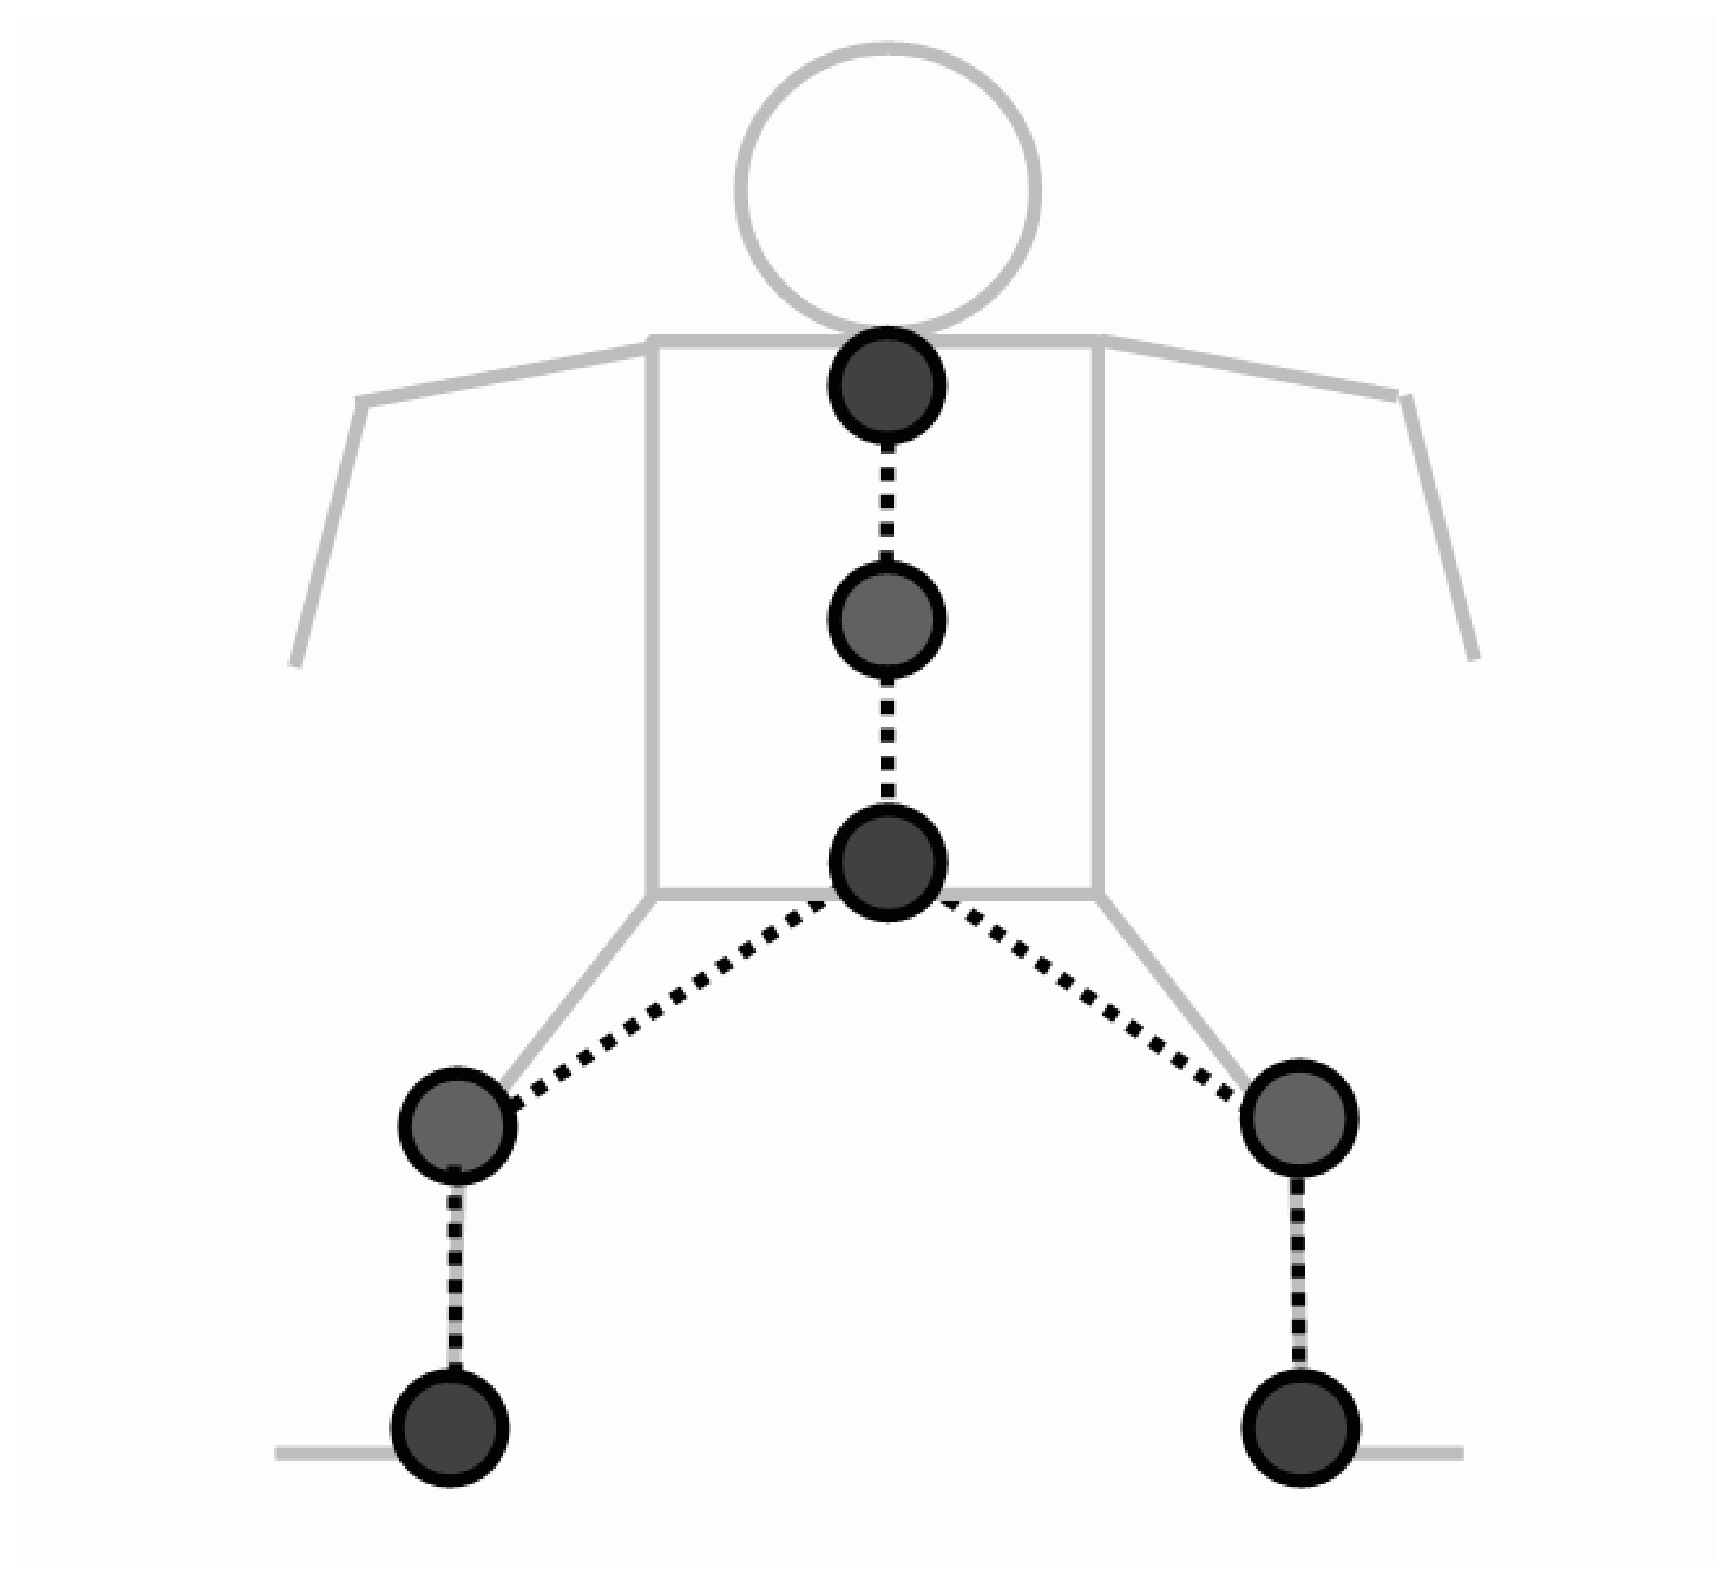
\includegraphics[width=5cm]{img/tags1}
%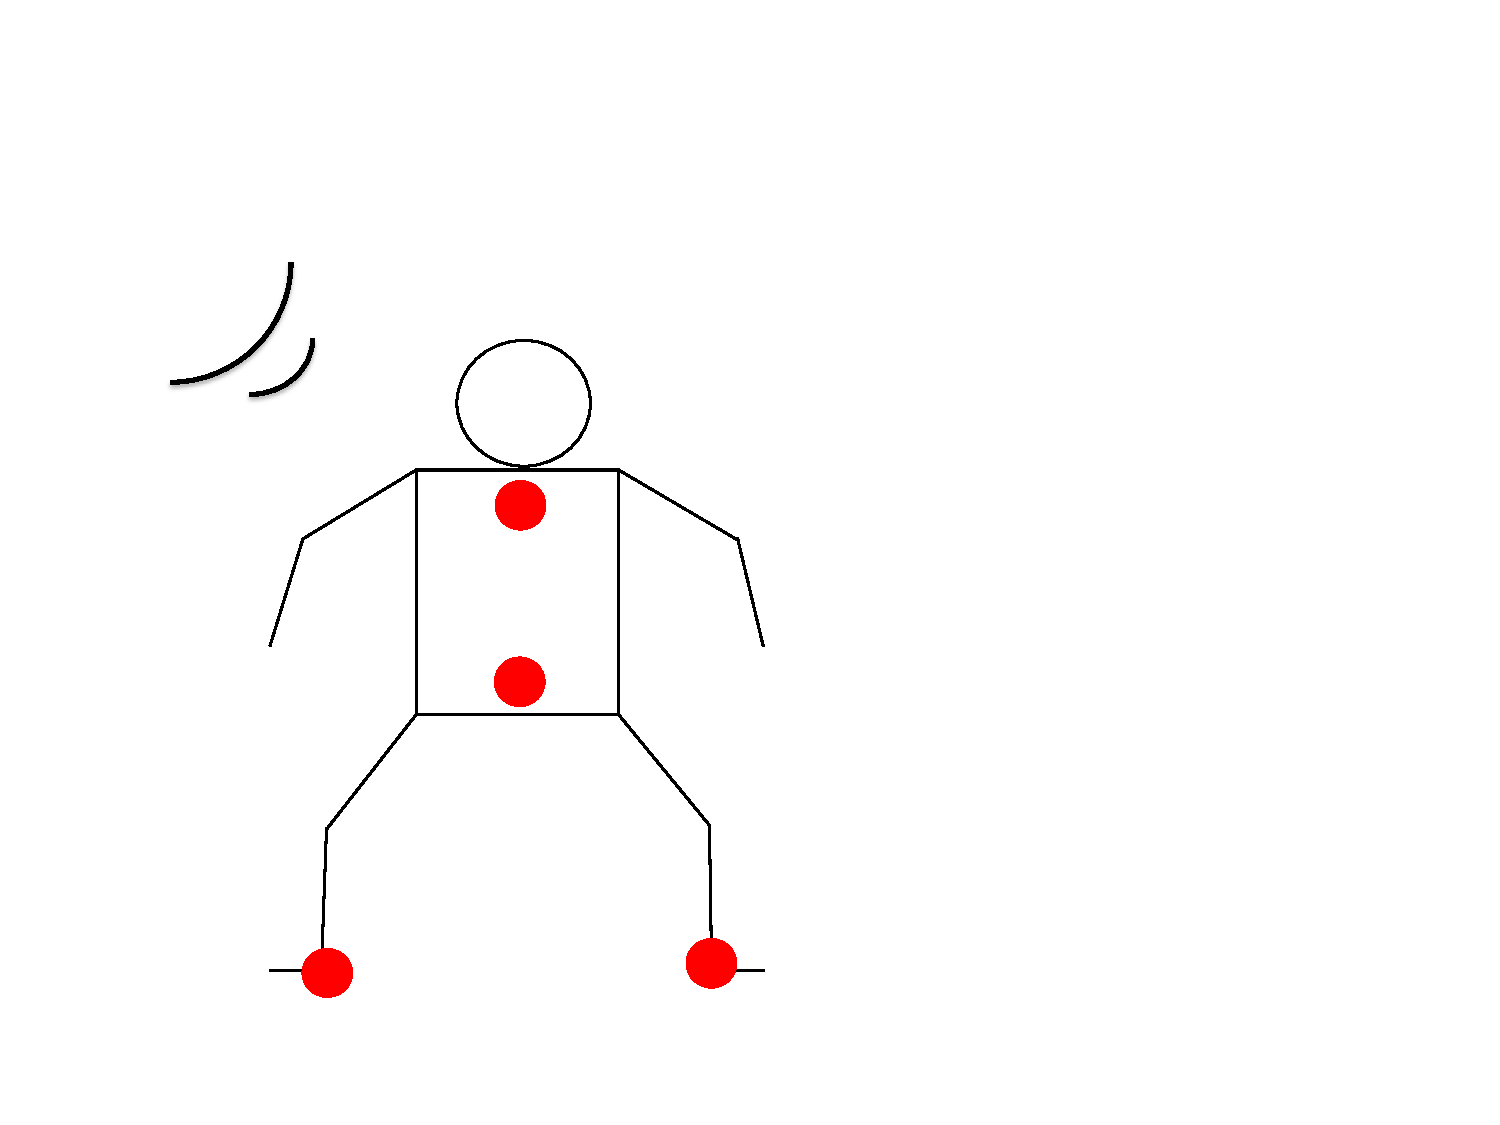
\includegraphics[bb=220 300 340 410, width=5cm]{img/tags.pdf}
\caption{Human body is modeled with an articulated rigid body.}
\label{fig:tags:noise}
\end{figure}

In our case, the four RTLS tags provide the joint positions (ankles, waist, and chest), but do not allow reconstructing the skeleton displayed in Figure~\ref{fig:tags:noise} since the knees and abdomen are missing. 

The missing joints are reconstructed as follows: suppose we have two points $A$ and $C$ with known positions and a joint $B$ that interconnects $A$ and $C$, with an unknown position. Since the distances $r_A=d(A, B)$ (between $A$ and $B$) and $r_c=d(C, B)$ are known, the point $B$ then lies at the intersection of two spheres, centered at $A$ with radius $r_A$ and at $C$ with radius $r_C$. 

In general, there are three cases when the measurements are obtained: (i) $r_A+r_B=d$, that is, the intersection includes a single point; (ii) $r_A+r_B>d$, that is, there is no solution; and (iii) $r_A+r_B<d$, that is, the intersection consists of a circle. In the second case we position the point $B$ on a line between points $A$ and $C$ so that the distances between points is in the same proportion as the lengths of $r_A$ and $r_B$.
%
In the third case, we proceed as follows: to calculate the position of the point $B$, we use a new coordinate system in which the first sphere is centered at the origin and the second sphere is centered at a point on the positive x-axis, at distance $d$ from the origin, as shown in Figure~\ref{fig:sphere-sphere}. Subtracting the sphere equations, we find a set of points representing a circular intersection of the spheres:
\begin{eqnarray}
\label{eq:circle}
x = \frac{d^2 - {r_C}^2 + {r_A}^2}{2d}, \\
\label{eq:circle1}
y^2 + z^2 = {r_A}^2 - (\frac{d^2 - {r_C}^2 + {r_A}^2}{2d})^2.
\end{eqnarray}
We are not interested in the exact position of B, hence we pick an arbitrary point from the circle and transform it to the original coordinate system.  As explained below, the distance between joints is enforced with Equations~(\ref{eq:fixDistance}) and (\ref{eq:fixDistance1}).

\begin{figure}[!h]
\centering
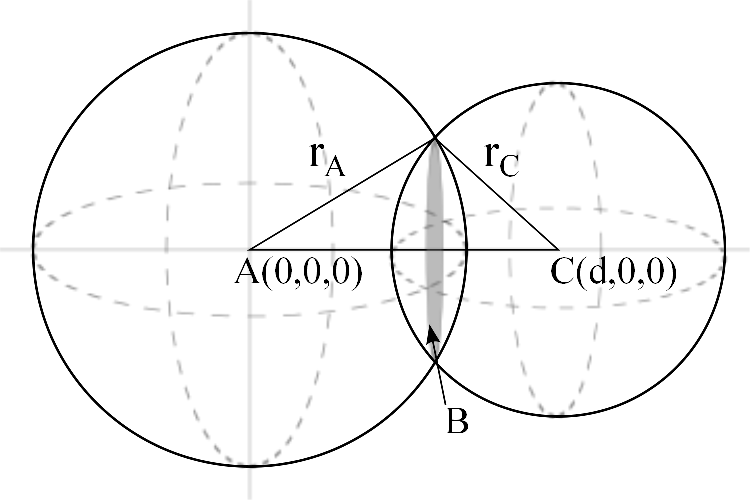
\includegraphics[width=0.5\textwidth]{img/sphere-sphere}
\caption{The result of sphere-sphere intersection is a circle.}
\label{fig:sphere-sphere}
\end{figure}

Once we have all the joint positions we can introduce constraints between the connected pairs. For example, suppose the true distance between joints A and  B is $r_A$, that is,
\begin{equation}
\label{eq:constraint}
\|\mathbf{p}_A - \mathbf{p}_B\| = r_A.
\end{equation}
If measurements $p_{A}$ and $p_B$ violate the constraint given by Equation~(\ref{eq:constraint}), the position of both points is adjusted \citep{Jakobsen2001}. 
%We differentiate two cases. In the first case, the measured distance is less than the true distance; that is, $d(p_A, p_B) < r_A$.
Each point is translated along the line connecting the points for half of the error defined as the difference between the measured and the true distance as shown in Figure~\ref{fig:distance-fix}. The update is:
\begin{eqnarray}
\label{eq:fixDistance}
\mathbf{p}'_A = \mathbf{p}_A + \frac{\|\mathbf{p}_B-\mathbf{p}_A\| - r_A}{2\|\mathbf {p}_B-\mathbf{p}_A\|}(\mathbf{p}_B-\mathbf{p}_A),\\
\label{eq:fixDistance1}
\mathbf{p}'_B = \mathbf{p}_B - \frac{\|\mathbf {p}_B-\mathbf{p}_A\| - r_A}{2\|\mathbf{p}_B-\mathbf{p}_A\|}(\mathbf {p}_B-\mathbf{p}_A).
\end{eqnarray}

\begin{figure}[!h]
\centering
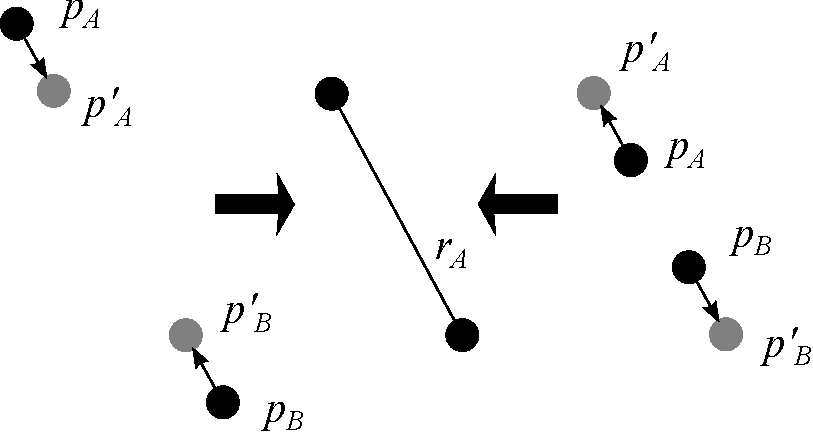
\includegraphics[width=0.5\textwidth]{img/distance-fix}
\caption{Move the points $\mathbf{p}_A$ and $\mathbf{p}_B$ to match the constraint given by Equation~(\ref{eq:constraint}).}
\label{fig:distance-fix}
\end{figure}

%Articulated rigid bodies & joint constraints


%\subsubsection{Spatio-Temporal Motion Patterns}
In addition to the constraints introduced by human body proportions, we also consider physical motion constraints such as velocity and acceleration, of limbs. Suppose that  $a$~m/s$^2$ is the greatest possible acceleration of an ankle. This implies that it can travel at most $l=(v_{t-1}+a\Delta t/2)\Delta t$ meters in time interval $\Delta t$, where $1/\Delta t$ is the sampling frequency. Hence, the next ankle's position $\mathbf{p}_{t}$ is limited with a sphere with radius $l$, that is, 
\begin{equation}
\|\mathbf{p}_{t} - \mathbf{p}_{t-1}\| \leq l.
\end{equation}
In case the new position is outside the sphere, the position is translated on the edge of the sphere in the direction of the measurement. The update step is:
\begin{equation}
\mathbf{p}'_t = \mathbf{p}_t + \frac{l (\mathbf{p}_t - \mathbf{p}_{t-1})}{\|\mathbf{p}_t-\mathbf{p}_{t-1}\|}.
\end{equation}


%image with sphere
%In order to speed up the computations we  approximate the sphere with a cube with edge length $l$. In this case we can limit the new position using Equation~\ref{eq:validDomain}. 


%\subsubsection{Iterative Constraint Relaxation}

Finally, all the constraints are put together. Consider $\mathbf{C}=\{\Phi_i\}$ as a set of constraints, where $\Phi(\mathbf{p})$ applies the update step on point $\mathbf{p}$ using Equation~(\ref{eq:validDomain}); that is, $\mathbf{p}' \leftarrow \Phi(\mathbf{p})$, while $\Phi(\mathbf{p}_A, \mathbf{p}_B)$ applies the update step on both points $A$ and $B$ using Equations~(\ref{eq:fixDistance}) and (\ref{eq:fixDistance1}); that is, $\mathbf{p}'_A, \mathbf{p}'_B \leftarrow \Phi(\mathbf{p}_A, \mathbf{p}_B)$.  If a constrained between points $A$ and $B$ is not present, then $\Phi(\mathbf{p}_A, \mathbf{p}_B)$ does not alter the corresponding points.
The algorithm below takes the set of constraints and its value updates as an input and iteratively updates the values until the convergence threshold $\tau_c$ or maximal number of iterations $k$ is reached.

\begin{algorithm}
\caption{Iterative constraint relaxation.}
\label{alg:LOF}
\begin{algorithmic}
\REQUIRE set of constraints $\mathbf{C}$, set of points $\mathbf{P}$, maximal number of iterations $k$, convergence threshold $\tau_c$
\ENSURE set of points $P$
\REPEAT
	\STATE $\Delta = 0$
	\FOR{$\mathbf{p} \in \mathbf{P}$}
		\FOR{$\mathbf{q} \in \mathbf{P}$}
			\STATE $\mathbf{p}', \mathbf{q}' \leftarrow \Phi(\mathbf{p}, \mathbf{q})$
			\STATE $\Delta \leftarrow \Delta + |\mathbf{q}-\mathbf{q}'|$
			\STATE $\mathbf{q} \leftarrow \mathbf{q}'$
		\ENDFOR
		\STATE $\mathbf{p}' \leftarrow \Phi(\mathbf{p})$
		\STATE $\Delta \leftarrow \Delta + |\mathbf{p}-\mathbf{p}'|$
		\STATE $\mathbf{p} \leftarrow \mathbf{p}'$
	\ENDFOR
	\STATE $k \gets k-1$
\UNTIL{$k > 0$ \AND $\Delta > \tau_c$}
\end{algorithmic}
\end{algorithm}


An example of filter effects is shown in Figure~\ref{fig:noise}, which shows $x$ (top), $y$ (middle) and $z$ (bottom) coordinates for a tag attached to the waist for $T=600$ time steps (one time step lasts approximately $1/8$ s). The vertical axis corresponds to meters. The blue line represents the original location measurements, the green line represents the median filter result, and the red line represents the Kalman filtering and spatial body constraints results.
\begin{figure}[!h]
\centering
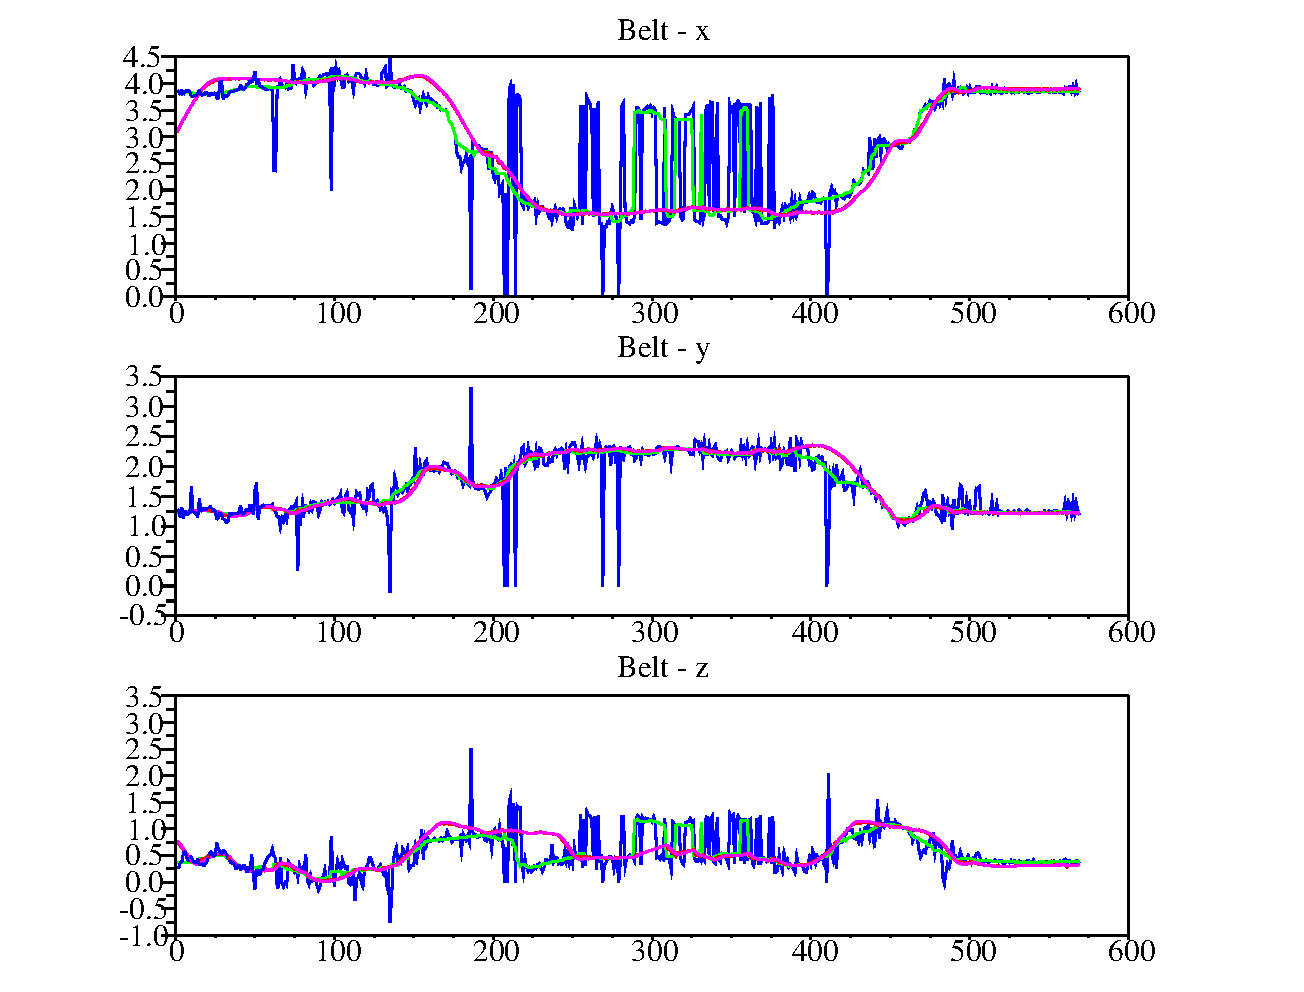
\includegraphics[width=0.85\linewidth]{chap_AR/cld-belt}
\caption{Filtered coordinates $x$ (top), $y$ (middle) and $z$ (bottom) of a tag attached to the waist.}
\label{fig:noise}
\end{figure}


%
%==========================================================================================
%
\section{Feature Vector}
\label{sec:ar:ml}

%The goal is to assign an activity $a$ from a set of possible actions in  $\mathbb{A}$ to an observation $x_t$. This section first discusses a 

%The goal of our research was to classify the person’s behavior into one of the following activities: falling, lying down, sitting down, standing/walking, sitting and lying. To obtain training data for a classifier to recognize these activities, we recorded 45 examples of the behavior of three persons. Each recording consisted of multiple activities:
%•	3 × 15 recordings of falling, consisting of standing/walking, falling and lying.
%•	3 × 10 recordings of lying down, consisting of standing/walking, lying down and lying.
%•	3 × 10 recordings of sitting down, consisting of walking, sitting down and sitting.
%•	3 × 10 recordings of walking.
%The recordings consisted of the coordinates of 12 body tags attached to the shoulders, elbows, wrists, hips, knees and ankles. This is the full complement of tags that will probably be reduced in the future. Since the equipment with which the Confidence system will acquire tag coordinates is still under development, the commercially available Smart infrared motion capture system [6] was used instead. The coordinates were acquired with 60 Hz. The frequency was afterwards reduced to 10 Hz, which is the expected Confidence data acquisition frequency. To make the recordings even more similar to what we expect of the Confidence equipment, we added Gaussian noise to them. The standard deviation of the noise was 4.36 cm horizontally and 5.44 cm vertically. This corresponds to the noise measured in the Ubisense real time location system [19]. The Ubisense system is similar to the equipment planned for acquiring tag coordinates in Confidence. The noise in the recordings was smoothed with Kalman filter [14].



%\subsection{Features}

Finding an appropriate representation of the person's activities is probably the most challenging part of activity recognition. The behavior needs to be represented with simple and general features, so that the model using these features will also be general and work well on behaviors different from those in the learning set. 
In fact, it is not difficult to design features specific to captured observations in a training set; such features would work well on them. However, since the training set captures only a part of the whole range of human behavior, overly specific features would likely fail on general behavior.

\begin{definition}
\label{def:feature}
	\emph{Feature vector} $\mathbf{f}_t$ at time step $t$ is a vector of descriptors obtained from observation $\mathbf{x}_t$. 
\end{definition}
\noindent
Feature $\mathbf{f}_t$ can hence contain values from observation as well as additional values computed from observation $\mathbf{f}_t$ or other observations. In general, the feature vector can be interpreted as observation extended with additional descriptors that capture targeted behavior.

\subsection{Features}

\index{feature extraction}
We propose three sets of features describing the person behavior in a selected domain. We demonstrate a possible feature set on a kinematic model of a human with 12 points as shown in Figure~\ref{fig:kinematic} to illustrate potential variety. In practice, however, it is possible to use a reduced feature set. First, reference features are expressed in the reference coordinate system, which is fixed with respect to the person's environment. Second, body features are expressed in a coordinate system affixed to the person's body. Third, angle features are the angles between adjacent body parts.

\begin{figure}[!h]
\centering
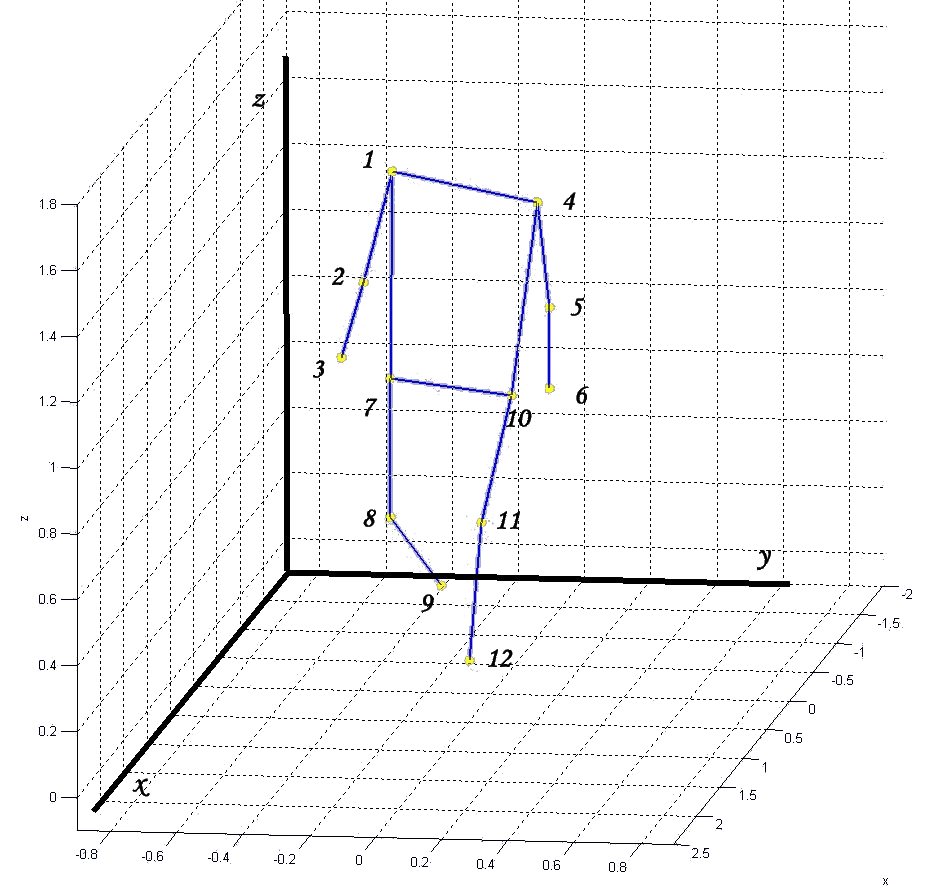
\includegraphics[width=0.7\linewidth]{chap_AR/kinematic_model}
\caption{Kinematic model of a human body.}
\label{fig:kinematic}
\end{figure}

\subsubsection{Reference Features}
When selecting reference features, the $x$ and $y$ coordinates are usually ignored, since these coordinates describe the person's location in the environment, but the activities of interest can generally take place at any location. A reasonable set of features can include $z^{(i)}_t$ coordinate of sensor tag $i$ at time $t$, the velocity of sensor tag in $z$ direction $v^{(i)}_t$, the absolute distance $d^{(i,j)}_t$between sensor tags $i$ and $j$, and others.


\subsubsection{Body Features}
Body features are expressed in a coordinate system affixed to the person's body. This makes it possible to observe $x$ and $y$ coordinates of the person's body parts, since these coordinates no longer depend on locations within the environment.

The body coordinate system is shown in Figure~\ref{fig:body_coordinate}. Its origin $\mathbf{o}$ is at the mid-point of the line connecting the hip tags ($\mathbf{p}_7$ and $\mathbf{p}_{10}$ in Figure~\ref{fig:body_coordinate}). This line also defines the $y$ axis, which points towards the left hip. The $z$ axis is perpendicular to the $y$ axis, touches the line connecting both shoulder tags ($\mathbf{p}_1$ and $\mathbf{p}_4$ in Figure~\ref{fig:body_coordinate}) at point $\mathbf{p}_z$, and points upwards. The $x$ axis is perpendicular to the $y$ and $z$ axes and points forwards.


\begin{figure}[!h]
\centering
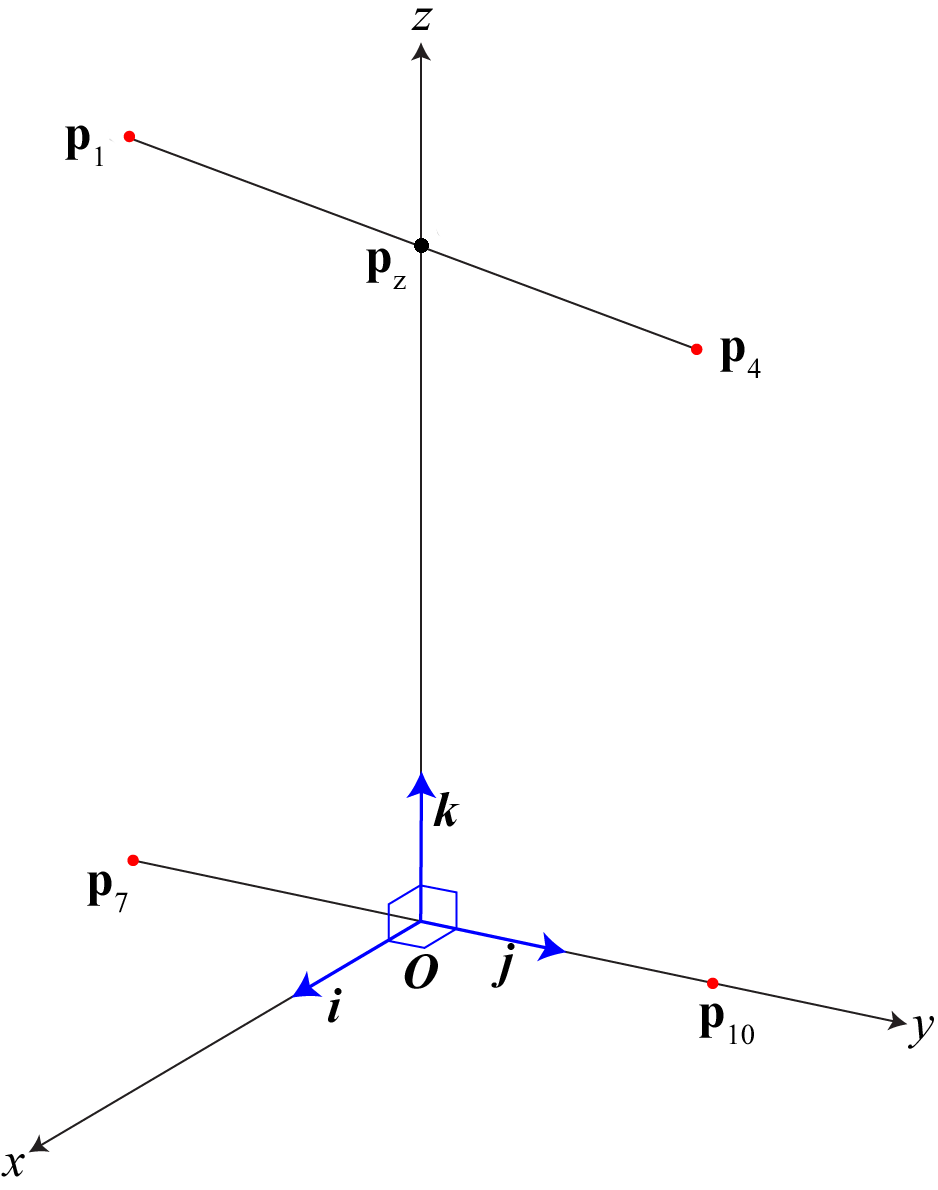
\includegraphics[width=0.5\linewidth]{chap_AR/body_coordinates}
\caption{The body coordinate system.}
\label{fig:body_coordinate}
\end{figure}

In order to translate reference coordinates into body coordinates, Equation~(\ref{eq:origin}) expresses the origin $\mathbf{o}$ and basis $(\mathbf{i}, \mathbf{j}, \mathbf{k})$ of the body coordinate system in the reference coordinate system, which gives us the basis vector $\mathbf{j}$:

\begin{equation}
\label{eq:origin}
\mathbf{o}=\frac{\mathbf{p}_7 + \mathbf{p}_{10} }{2},
\end{equation}

\begin{equation}
\label{eq:basis_j}
\mathbf{j}=\frac{\mathbf{p}_7 - \mathbf{o} }{|\mathbf{p}_{10} - \mathbf{o}|}.
\end{equation}

\noindent
To obtain the basis vector $\mathbf{k}$, Equation~(\ref{eq:p_z}) is first used to calculate $\mathbf{p}_z$; Equation~(\ref{eq:basis_k}) then gives us $\mathbf{k}$:
\begin{equation}
\label{eq:p_z}
\mathbf{p}_z = \mathbf{p}_7 + a(\mathbf{p}_4 - \mathbf{p}_7),
\end{equation}

\begin{equation}
a 	= \frac{(\mathbf{p}_1 - \mathbf{o}) \cdot (\mathbf{p}_{10} - \mathbf{p}_7)}{(\mathbf{p}_4 - \mathbf{p}_1) \cdot  (\mathbf{p}_{10} - \mathbf{p}_7)},
\end{equation}

\begin{equation}
\label{eq:basis_k}
\mathbf{k}=\frac{\mathbf{p}_7 - \mathbf{o} }{|\mathbf{p}_{10} - \mathbf{o}|}.
\end{equation}

Finally, we obtain basis vector $\mathbf{i}$ using Equation~(\ref{eq:basis_i}):
\begin{equation}
\label{eq:basis_i}
	\mathbf{i}=\mathbf{j} \times \mathbf{k}.
\end{equation} 

	 
To translate a point $\mathbf{p}$ coordinates in the reference coordinate system into the body coordinate systems, Equation~(\ref{eq:transform}) is used. The vector $\mathbf{p}_R = (x_R, y_R, z_R, 1)$ corresponds to the point $\mathbf{p} = (x, y, z)$ in the reference coordinate system. The vector $\mathbf{p}_B = (x_B, y_B, z_B, 1)$ corresponds to the point $\mathbf{p}=(x_B, y_B, z_B)$ in the body coordinate system. Matrix $\mathbf{T}_{R \rightarrow B}$ is the transformation matrix from the reference to the body coordinate system. 

\begin{equation}
\label{eq:transform}
\mathbf{p}_B=\mathbf{T}_{R \rightarrow B} \mathbf{p}_B^\intercal,
\end{equation} 
$$
 \mathbf{T}_{R \rightarrow B} = \begin{bmatrix}
        \mathbf{i}_x &	\mathbf{i}_x &	\mathbf{i}_x &	-\mathbf{o} \cdot \mathbf{i} \\
        \mathbf{j}_x &	\mathbf{j}_x &	\mathbf{j}_x &	-\mathbf{o} \cdot \mathbf{i} \\
        \mathbf{k}_x &	\mathbf{k}_x &	\mathbf{k}_x &	-\mathbf{o} \cdot \mathbf{i} \\
        0 &	 			0 &				0 &				1
      \end{bmatrix}.
$$

Based on the above equations, a reasonable set of body attributes may include the tag's body features, absolute velocity, and the angles of movement with respect to the $z$ axis and $xz$ plane, and others.

\subsubsection{Angle Features}	

Once the body coordinate system is obtained, it is possible to compute an advanced set of features describing relative angles between different body parts represented by quaternions. Unit quaternions provide a convenient mathematical notation for representing object orientations and rotations in three dimensions. Compared to Euler angles, they are simpler and avoid the gimbal lock problem. Compared to the rotation matrices, they are more efficient and numerically stable. %Quaternions have found their way into applications in computer graphics, robotics, navigation, and orbital mechanics of satellites. 

This thesis will not go into further details on angle equations; the reader is referred to \cite{Lustrek2008report} for details. A reasonable set of attributes may include the angles of the left and right elbow, the left and right knee, the left and right shoulder (represented by quaternions), the left and right hip (also represented by quaternions), and others.


\subsection{Canonical Representation}
\index{canonical representation}
Due to its continuous nature, determining the exact transition points between activities is difficult. We address this issue by combining features into short, overlapping time windows during which we assume that a single activity is dominant. We denote this representation as canonical form that represents the equivalence classes. To test whether two activities in specific time interval are equivalent, it suffices to test their canonical forms for equality. A canonical form thus enables classification and gives a distinguished (canonical) representative of an action.

In practical terms, one wants to be able to recognize the canonical forms; that is, overlapping windows. Each window is classified independently as described in the next section (Section~\ref{sec:ArModel}).

More formally, we define:
\begin{itemize}
	\item $w$ is window length that contains an even number of observations,
	\item $i$ is an index over $|w|$ elements in window, and
	\item $j$ is an index over $W$ overlapping windows.
\end{itemize}

Given a sequence of observations $\{\mathbf{x}_1, \mathbf{x}_2, ..., \mathbf{x}_T\}$, we first compute the sequence of features $\{\mathbf{f}_1, \mathbf{f}_2, ..., \mathbf{f}_T\}$. Then, for constants $m$ and $n$, where $m$ is the number of elements before $t$, and $n$ after $t$; that is, $m+n=|w|+1$, we construct $W_j$, $1 \leq j \leq (|T|-|w|+1)$ windows such that
\begin{equation}
\label{eq:window}
W_j = \{\mathbf{f}_i | j - m \leq i \leq j + n \}.
\end{equation}
Each $W_j$ is labeled with a dominant activity from $\mathbb{A}$ that is assigned to the feature vector $\mathbf{f}_t$. Note, that Equation~(\ref{eq:window}) allows $\mathbf{f}_t$ to adopt any position in $W_j$; in practice it is placed at the beginning ($m=0$), middle ($m=n$), or at the end ($n=0$).
%
An example for $w=9$ and $m=n=4$ is shown in Figure~\ref{fig:canonical}. First, each feature vector is constructed by three sets of attributes. Then, the vector is presented in canonical representation with a window. The end of the window is labeled with the dominant activity.
%observation are captured for 10 time steps and extended to feature vectors. ...

\begin{figure}[!h]
\centering
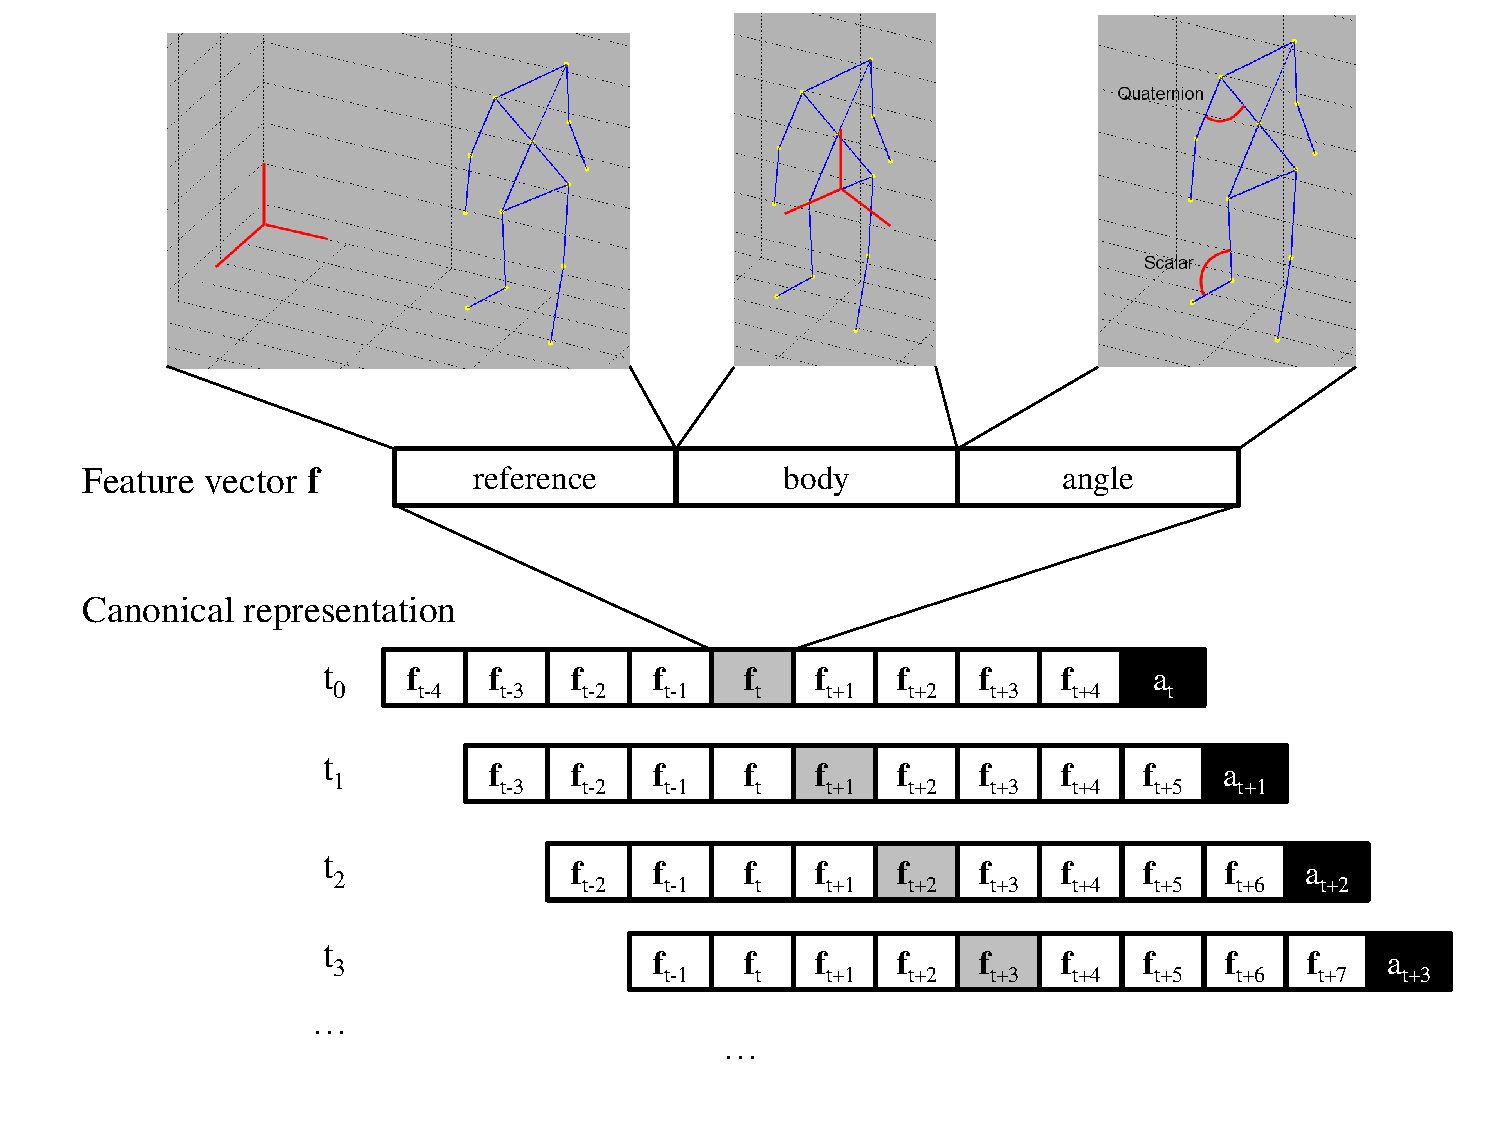
\includegraphics[width=\linewidth]{chap_AR/features}
\caption{An example of 10 feature vectors in canonical representation.}
\label{fig:canonical}
\end{figure}

The intuition behind the canonical representation is that an agent's actions are continuous and, hence, defined not only by the current values but also by the values in a certain time span. 
%Window length is chosen manually; long window length may lead to high 
So far, the features were expressed in corresponding coordinate systems at each time step $t$. However, the features $\mathbf{f}_i$ at time steps $i \not= t$ in the canonical representation can be expressed in the coordinate system belonging to the feature at time step $t$. This explicitly captures the changes between time steps within the interval. 





\subsection{Activity Recognition Model}
\label{sec:ArModel}
%\subsection{Results}
Once feature vectors are represented in the canonical form, it is possible to apply standard techniques for supervised classification, including feature selection, feature discretization, model learning, $k$-fold cross-validation, etc. The thesis will not delve into the details of the machine-learning algorithms. Any algorithm that supports numerical features can be applied to canonical representation, including SVMs, random forest, AdaBoost, decision trees, neural networks, multi-layer perceptrons, and others.

An important note considers $k$-fold cross-validation. Overlapping windows have a large degree of similarity and hence straight-forward $k$-fold cross-validation may produce an optimistic estimate of model performance. A better approach is to use folds that correspond to different sets of measurements or even different agents. For example, if the available dataset contains measurements of five agents, it makes sense to run {\it k-agent} cross-validation, where the model is trained on four agents and tested on the fifth.  The procedure is repeated for each agent and results are averaged.

%Activity recognition may be enhanced by appending A previous activities as recognized by the classifier to the attribute vector. This is particularly relevant in the first case where only a single set of attributes is used. The danger of appending previous activities is that the machine learning algorithm may learn that the current activity is always the same as the previous one, since this will often be the case. The problem may be circumvented by having two classifiers CA and C0. CA’s attribute vector contains A previous activities as recognized by C0. C0’s attribute vector does not contain any previous activities. This way even if CA gives a lot of weight to previous activities, the previous activities as recognized by C0 will change, as C0 is not burdened with CA’s inertia.

%
%==========================================================================================
%
\section{Reducing Spurious Activity Transitions}
\label{sec:ar:spurious}

\index{spurious activity transitions}
\index{noise removal}
An activity-recognition model classifies each window into one of the predefined activities; however, regardless of our efforts, it may still mislabel activities. The model usually mislabels single moments or short intervals more often than longer intervals. Activity recognition can be improved by taking into account the continuity of activities, for example, the agent cannot switch between walking and lying every tenth of a second. Such transitions between activities that do not occur in reality, but are caused by mislabeling, are considered spurious. 

One approach to enhancing the activity recognition model is to the extend feature vector with $k$ previous activities as recognized by the classifier. This leads to a potential problem, namely, the machine-learning algorithm may learn that the current activity is always the same as the previous one, since this is often the case. The problem may be circumvented by having two activity recognition models $\theta_A$ and $\theta$, where $\theta_A$'s attribute vector does not contain any previous activities, and $\theta$'s attribute vector contains $k$ previous activities as recognized by $\theta_A$. This way, even if $\theta$ heavily weights previous activities, those  recognized by $\theta_A$ will change, as $\theta_A$ is not biased with $\theta$'s inertia.

Based on the above intuition, we introduce two candidate approaches for reducing spurious activity transitions: sequential grammar-based classifier (SGBS) and hidden Markov models (HMM).  The input to these models is a sequence of actions $\mathbf{a}$ labeled by an activity recognition model $\theta_A$. 
\begin{definition}
\index{action!action sequence}
	\emph{Activity sequence} $\avec{T}$ is a totally-ordered sequence of $T$ actions s.t. $\avec{T}=\{a_t; 1 \leq t \leq T\}$.
\end{definition}
\noindent
The goal is to assign the best possible sequence of actions $\mathbf{a}'$ given a criterion and a sequence of input actions $\mathbf{a}$, often referred to as an observation sequence.


\subsection{Sequential Grammar-Based Classifier}

\index{sequential grammar-based classifier}
A sequential grammar-based classifier, introduced by \cite{Goshorn2001}, classifies an observed activity sequence $\mathbf{a}$ to the behavior which it most closely resembles. The similarity is defined in terms of the transformation cost of a sequence into a syntactically correct sequence belonging to that behavior. 

Suppose there is a set of $n$ possible behaviors $\mathbf{b}_i \in \mathbb{B}$, $1 \leq i \leq n$. A behavior $\mathbf{b}_i$ consists of a sequence of actions $a \in \mathbb{A}$ and is generated with a corresponding finite state machine $M_i(\mathbb{A}, S, s_o, \delta, F)$, where $\mathbb{A}$ is the input alphabet (activities), $S$ is a finite, non-empty set of states, $s_0$ is an initial state, $\delta: S \times \mathbb{A} \rightarrow S$ is state-transition function, and $F$ is the set of final states.


Suppose you want to classify an observation sequence $\avec{k}=\{a_1, a_2, ..., a_k\}$. If $\avec{k}$ is recognized by any of the automata $M_i$, then it is classified as behavior $\mathbf{b}_i$. If it is not, then it must be edited into a sequence that is. In order to do so, a new automaton $M'_i$ is created, which is able to parse unrecognizable sequence $\avec{k}$ by transforming any symbol within its alphabet, but with an associated cost, as follows. There are two operations that are used for transformations: substitution and deletion. Let $S(a_i, a_j)$ denote the operation of substituting an input symbol $a_i$ with $a_j$, and let $D(a_i)$ denote the operation of deletion of symbol $a_i$. Denote edit costs as $c_S(a_i, a_j)$ and delete cost $c_D(a_i)$, respectively. 

In order to utilize the performance of the classifier $\theta_A$, we use its performance measures obtained from its confusion matrix. The error rate for mislabeling an activity $a_i$ with $a_j$ is relevant for assigning the cost of substituting action $a_i$ with $a_j$. Therefore, to derive $c_S(a_i, a_j)$, we simply invert the probability $\Prob\{a_i|a=a_j\}$ from the confusion matrix:
\begin{equation}
\label{eq:sgbc}
c_S(a_i, a_j) = \frac{1}{\Prob\{a_i|a=a_j\}}.
\end{equation}

Similarly, the cost for deleting the action $a_i$ is defined inversely proportional to the inherent probability that classifier $\theta_A$ labels $a_i$ with true activity correctly. The deletion cost $c_D(a_i)$ is:
\begin{equation}
\label{eq:sgbc}
c_D(a_i) = \frac{1}{\Prob\{a_i|a=a_i\}}.
\end{equation}

Suppose, that in order to transform the action sequence $\avec{k}$ into a behavior $\mathbf{b}_i$, there need to be $n_S(a_i, a_j)$ substitutions of $a_i$ with $a_j$ and $n_D(a_i)$ deletions of $a_i$. Then, the distance $d(\avec{k}, \mathbf{b}_i)$ between the action sequence $\avec{k}$ and a behavior $\mathbf{b}_i$ is given by Equation~(\ref{eq:sgbc}):
\begin{equation}
\label{eq:sgbc}
d(\mathbf{a}, \mathbf{b}_i) = \sum_{i=0}^{|\mathbb{A}|} \sum_{j=0}^{|\mathbb{A}|} c_S(a_i, a_j) n_S(a_i, a_j) + \sum_{i=0}^{|\mathbb{A}|} c_D(a_i) n_D(a_i).
\end{equation}

The action sequence $\avec{k}$ is classified as a behavior $\mathbf{b}_i$ represented by a finite state machine $M_i'$ that outputted the smallest distance:
\begin{equation}
\label{eq:sgbc-argmin}
\mathbf{a} = \argmin{\mathbf{b}_i \in \mathbb{B}} d(\mathbf{a}, \mathbf{b}_i).
\end{equation}

In general, the lengths of behaviors $\mathbf{b}_i$ and action sequence $\mathbf{a}$ need not be be the same (although the lengths of behaviors $\mathbf{b}_i$ should be in to avoid length normalization). 
To avoid this problem,
%we can initialize one behavior $b$ for each action from $\mathbb{A}$. Then, given the input sequence $\mathbf{a}$, 
we use the overlapping sliding windows of length $|\mathbf{b}|$ and assign the classified behavior to the activity at the selected window index.



\subsection{Hidden Markov Models} 
\label{sec:ar:hmm}

\index{hidden Markov models}
Hidden Markov model (HMM) is a temporal probabilistic model with two embedded stochastic processes: a hidden process $Q$ that can be observed only through another visible process $O$. Each state has state-transition probabilities, which are visible, and a probability distribution over the possible values of $\mathbb{A}$. The key assumption is that the current hidden state of the agent is affected only by its previous state.  

A hidden Markov model $\theta(\mathbb{H}, \mathbb{A}, \delta, \nu, \pi)$ is characterized by the following:
\begin{itemize}
	\item $\mathbb{H}=\{h_i\}$ is a set of $N$ hidden states, individual states are denoted as $\mathbb{H}=\{h_1, h_2, ..., h_N\}$, and the state at time $t$ as $Q_t$,
	\item $\mathbb{A} = \{a_j\}$ is a set of distinct observation symbols (that is, activities) per state,
	\item $\delta = \{\delta_{ij}\}$ is the state transition probability distribution, where 
		\begin{equation}
			\label{eq:hmm-a}
			\delta{ij} = \Prob\{q_{t+1} = s_j | q_t = h_i\}, 1 \leq i,j \leq N,
			\end{equation}
	\item $\nu = \{\nu_{j}(k)\}$ is the state observation probability distribution, where 
			\begin{equation}
			\label{eq:hmm-b}
			\nu_{j}(k) = \Prob\{a_k | q_t = h_j\}, 1 \leq j \leq N, 1 \leq k \leq M, 
			\end{equation}
	\item $\pi=\{\pi_i\}$ is the initial state distribution, where
			\begin{equation}
			\label{eq:hmm-pi}
			\pi_i = \Prob\{q_1 = h_i\}, 1 \leq i \leq N.
			\end{equation}
\end{itemize}
\noindent An example of a hidden Markov model with $N=4$ hidden states and $M=3$ observation symbols is shown in Figure~\ref{fig:hmm}. 

\begin{figure}[!h]
\centering
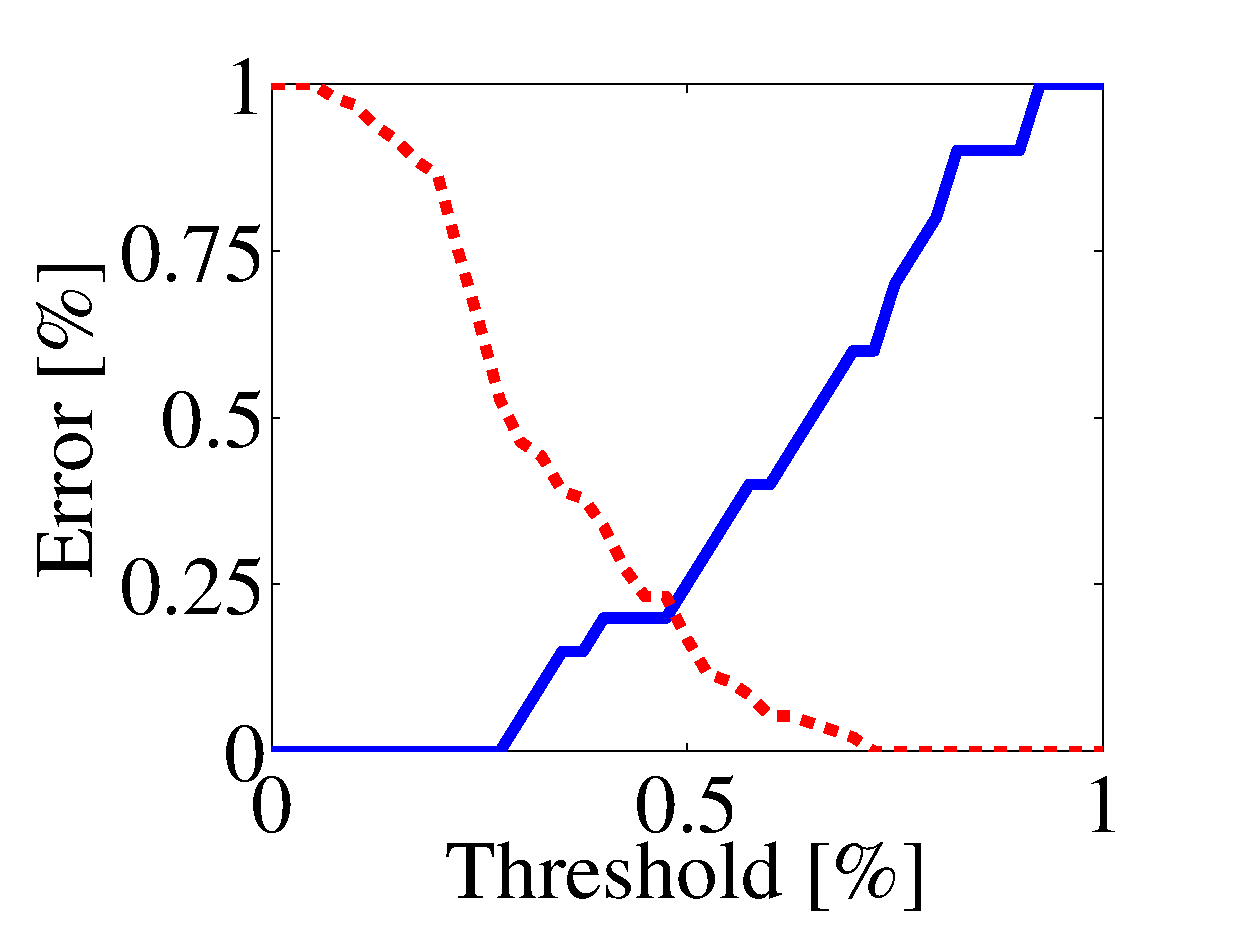
\includegraphics[width=\linewidth]{chap_AR/hmm}
\caption{An example of a hidden Markov model with four hidden states and three observation symbols.}
\label{fig:hmm}
\end{figure}

Given a learning set of observation sequences, there are two problems of interest that must be solved; that is, how to adjust model parameters so as to best describe agent behavior observation sequences, and, given a new observation sequence $\mathbf{a}^{(t)}$ and a model $\theta$, how to choose a corresponding state sequence $\mathbf{s} = \{q_i=h_j | 1 \leq i \leq t, 1 \leq j \leq M\}$, that best explains the observations.

%Consider a model $\theta$ characterized with $N$ hidden states, denoted as $S1, S2, …, SN$. Let aij denote state transition probability from state Si to Sj and let πi denote initial state distribution of state Si. Denote M as the number of distinct output symbols s1, s2, …, sm and output symbol distribution in state j as bj(k). Then, given appropriate values N, M, aij, πi, and bj(k), the HMM can be used as generator of output sequence s=s1s2s3…sk.

The first problem, where the goal is to adjust model parameters in order to maximize observation sequence probability, has no optimal solution. Parameters can be locally maximized with the Baum-Welch method~\citep{Baum1970}, which maximizes the likelihood of the training set. Instead of calculating the required state transitions from the observations, it iteratively estimates the parameters. The method starts with arbitrarily chosen values and then computes the expected frequencies by weighting the observed sequences over the current model probabilities. The expected frequencies substitute the old parameters and the procedure iterates until converging on a local maximum. 

The second problem, {\it uncovering} the hidden part of the model, is solved with the Viterbi algorithm~\citep{Viterbi1967}, which assumes that the output symbols in observation sequence $\mathbf{a}$ correspond to hidden state sequence $\mathbf{h}$. It finds the optimal state sequence $\mathbf{h}$ for the given observation sequence $\mathbf{a}$ in terms of maximizing the expected number of correct states, which is achieved with dynamic programming.

Suppose the task is to classify an observation sequence $\mathbf{a}$. First, an HMM model $\theta$ is created from the learning set of observations with the Baum-Welch method. Then, the Viterbi algorithm applied on model $\theta$ and observation sequence $\mathbf{a}$ returns the most probable hidden state sequence $\mathbf{h}$. In the last step, we take into account the $\theta$'s state observation probability distribution $\nu$ to assign the most probable symbol to each state; that is, it is assumed that a hidden state corresponds to the activity that is most likely observed in that state.

%
%==========================================================================================
%
\section{Compound-Activity Recognition}
\label{sec:ar:interactions}

\index{activity!compound activity}
We use the term compound activity to describe behavior within an activity sequence. %; that is, it describes behavior of an agent in a longer time interval 
Activities, in particular atomic actions, are mainly used as behavior primitives describing the most elementary behavior aspects, while compound activities describe higher-level behavior aspects, usually spanned over longer periods of time.

\begin{definition}
\label{def:compound_activity}
\index{interaction}
	\emph{Compound activity} $b_k \in \mathbb{B}$ describes an activity sequence $\avec{k}$ as behavior caused by an agent in a particular situation limited by time span $1 \leq t \leq k$ that explains activities $a_1, ..., a_k$, where $\mathbb{A}$ is a set of possible activities.
\end{definition}

The main difference between activities and compound activities is in the mapping function: an activity is assigned from observation vector(s), that is, $f: \mathbb{R}^{|\mathbf{x}|} \rightarrow \mathbb{A}$, while a compound activity is assigned from an activity sequence, that is, $g: \mathbb{A}^{|\avec{k}|} \rightarrow \mathbb{B}$. Given a set of possible compound activities $\mathbb{B}=\{b_i\}, 1 \leq i \leq K$, the goal is to classify an activity sequence $\mathbf{a}$ into one of the activities from $\mathbb{B}$.

For this task, we utilize hidden Markov models introduced in the previous section. The idea is to segment the learning set by different behavior types and to create an HMM model $\theta_i$ for each of the behaviors $b_i \in \mathbb{B}, 1 \leq i \leq K$.

Next, we compute the probability of the sequence $\mathbf{a}$ given a model $\theta_i$, that is, $P[a|\theta_i]$. The straightforward approach through enumerating every possible state sequence of length $T=|\mathbf{a}|$ involves the order of $2TN^T$ calculations~\citep{KollerFriedman2009}, which is computationally unfeasible even for small values of $N$ and $T$, for example, $N=5$ states and $T=100$ requires $~10^{72}$ calculations. A more efficient procedure, denoted as the forward-backward algorithm~\citep{Rabiner1989}, first computes a set of forward probabilities that predicts the likelihood of ending up in any particular state given the first $t$ observations in the sequence $\mathbf{a}$. In the second pass, the algorithm computes a set of backward probabilities that predicts the likelihood of the remaining observations given any starting point $t$. These two probability distributions can then be combined to obtain the distribution over states at any specific point in time given the entire observation sequence. The reader is referred to \cite{KollerFriedman2009} for details.

Finally, the atomic action sequence $\mathbf{a}$ is classified as the behavior $b_i$ that outputted the highest probability $\Prob\{\mathbf{a}|\theta_i\}$:
\begin{equation}
\label{eq:hmm-max}
\argmax{b_i \in \mathbb{B}} \Prob\{\mathbf{a}|\theta_i\}.
\end{equation}

%
%==========================================================================================
%
\section{Recognition of Agent-Agent Interactions}
\label{sec:ar:interactions}
\index{activity!compound activity}
The previous sections were mainly focused on single-agent behavior. In order to assess all the behavior aspects, some domains require recognition of interactions among agents.

\begin{definition}
\label{def:observation_vector}
\index{interaction}
	\emph{Interaction} between agents $A$ and $B$ or interactive behavior $\chi_{i, j}(\tuple{\mathbf{a}_A,\mathbf{a}_B}) \in \mathbb{I}$ is behavior in time span $i \leq t \leq j$ that explains activity sequences $\mathbf{a}_A$ and $\mathbf{a}_B$ that correspond to activity sequence of the agent $A$ and agent $B$, respectively. $\mathbb{I}$ is a set of possible interactions.
\end{definition}

\noindent In other words, an interaction describes joint behavior of two agents in a specific time span. 

\index{hidden Markov models!coupled hidden Markov models}
This section demonstrates an approach for interaction recognition based on coupled hidden Markov models (CHMMs), which are briefly described below. The reader is referred to \cite{Brand} for details. The observation sequence $\hat{\mathbf{a}}=\tuple{\mathbf{a}_A, \mathbf{a}_B}$ consists of two activity sequences, namely $\mathbf{a}_A$ of agent $A$ and $\mathbf{a}_B$ of agent $B$, when they are within some predefined radius $R$. The CHMMs are able to model complex, interactive behavior by two HMM chains, where the hidden states from one chain directly impact the hidden states from the other chain. 

Figure~\ref{fig:CHMMs} illustrates a CHMM for a pair of action traces with length $l=3$. The current state $Q_t^A$ of agent $A$ is affected by both its previous state $Q_{t-1}^A$ and previous state $Q_{t-1}^B$ of the agent $B$ (similarly $Q_t^B$ is affected by $Q_{t-1}^B$ and $Q_{t-1}^A$). Each state $Q_i$ also impacts the corresponding observation state $Y_t$. 
For example, if agent $A$ moves toward agent $B$, the next state of the latter takes this into account and produces a corresponding atomic action, for example, an avoidance maneuver. 

\begin{figure}[!ht]
\centering
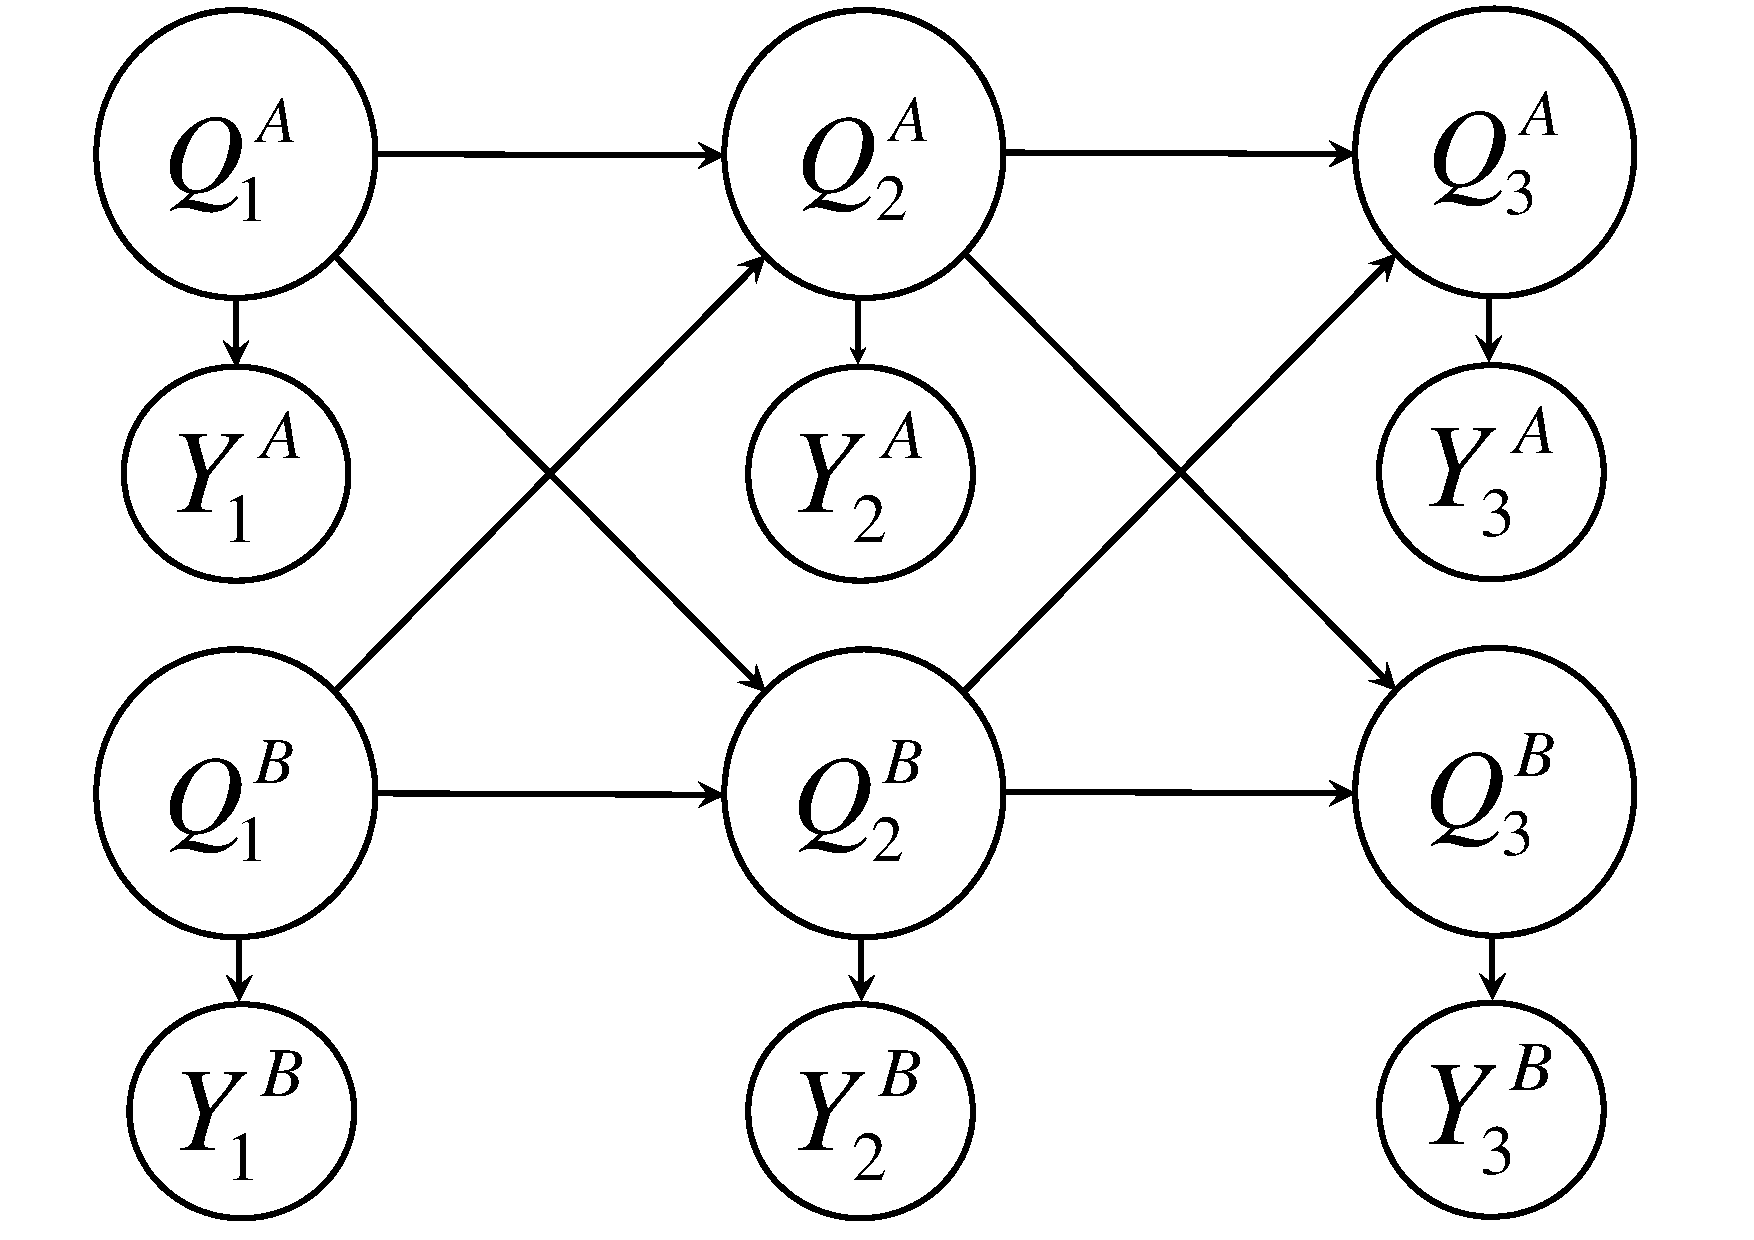
\includegraphics[width=0.5\linewidth]{chap_AR/chmm}
\caption{An example of CHMM for a pair of action traces with length $T=3$.}
\label{fig:CHMMs}
\end{figure}

Similarly to the previous section, we create a CHMM model $\hat \theta_i$ for each interaction $\chi_i$ from the set of possible interactions $\mathbb{I}$. For an observation sequence $\hat{\mathbf{a}}$, the posterior probability is computed given the model $\hat \theta_i$ using slightly modified standard HMM algorithms. The reader is referred to \cite{Brand} and \cite{KollerFriedman2009} for details.
Finally, the interaction is classified by the model that outputs the highest probability $\Prob\{\hat{\mathbf{a}}|\hat \theta_i\}$:
\begin{equation}
\label{eq:chmm-max}
\argmax{\chi_i \in \mathbb{I}} \Prob\{\hat{\mathbf{a}}|\hat \theta_i\}.
\end{equation}


\section{Summary and Discussion}
This chapter addressed the activity recognition from sensor data, where considerable amount of noise is present. We introduced a pipeline-based approach, ARPipe, that includes noise removal, feature vector construction, activity recognition classifier, and spurious activity transition removal. The noise removal as well as feature vector construction steps were demonstrated on location-based sensors, which provide significantly less accurate measurements compared to location sensors used in related work \citep{Sukthankar2005, Qian2004}. Since real locations, that is, true locations of a moving object, were infeasible to obtain, the noise removal was evaluated indirectly in \citep{Kaluza2009Glajenje, Lustrek2009Behavior}, where it proved beneficial. The removal of spurious activity transitions was investigated in \citep{Kaluza09Reducing}, where HMM approach achieved better results. In summary, the main two novelties presented in this chapter are activity recognition from noisy location sensors, and the ARPipe, which represents a comprehensive approach to activity recognition.

ARPipe provides the fist step to anomalous and suspicious behavior detection by recognizing behavior primitives, that is, activities. Additional approaches, such as compound activity recognition and recognition of agent interactions, help us to recognize more complex behaviors. The next chapter will discuss how to encode and evaluate such behavior components.




